%--------------------
% Packages
% -------------------
\documentclass[11pt,a4paper,titlepage]{article}
\usepackage[utf8x]{inputenc}
\usepackage[T1]{fontenc}
%\usepackage{gentium}
\usepackage{mathptmx} % Use Times Font


\usepackage[pdftex]{graphicx} % Required for including pictures
\usepackage[english]{babel} % Swedish translations
\usepackage[pdftex,linkcolor=black,pdfborder={0 0 0}]{hyperref} % Format links for pdf
\usepackage{calc} % To reset the counter in the document after title page
\usepackage{enumitem} % Includes lists

\frenchspacing % No double spacing between sentences
\linespread{1.2} % Set linespace
\usepackage[a4paper, lmargin=0.1666\paperwidth, rmargin=0.1666\paperwidth, tmargin=0.1111\paperheight, bmargin=0.1111\paperheight]{geometry} %margins
%\usepackage{parskip}

\usepackage[all]{nowidow} % Tries to remove widows
\usepackage[protrusion=true,expansion=true]{microtype} % Improves typography, load after fontpackage is selected

%-----------------------
% Set pdf information and add title, fill in the fields
%-----------------------
\hypersetup{ 	
pdfsubject = {},
pdftitle = {},
pdfauthor = {}
}

%-----------------------
% Begin document
%-----------------------

\begin{document} %All text i dokumentet hamnar mellan dessa taggar, allt ovanför är formatering av dokumentet
\bibliographystyle{ieeetr}

\begin{titlepage}
  \centering
  \vspace*{2cm}
  {\Huge \textbf{\underline{CS-E4840}}}\\[0.5cm]
  {\Huge \textbf{\underline{\parbox{0.8\linewidth}{\centering Information Visualization D}}}}\\
  [2cm]
  {\Large Aleksi Kääriäinen (728971)}\\[0.5cm]
  {\Large \today}
\end{titlepage}

\section{Getting Started}

\subsection{SDG Selection}
\begin{enumerate}
    \item The website available at \cite{sdgs} lists \textbf{The Sustainable Development Goals} introduced by the United Nations as part of the 2030 Agenda for Sustainable Development. In total, it contains 17 goals. I selected goal number 1, i.e. the \textbf{No Poverty} goal, for the subject of visualization in this assignment.
    \item I selected the goal because it is concrete and measurable, unlike some of the other goals listed. For example, the United Nations \cite{endpov} defines the extreme poverty line to be a daily income of less than US\$2.15. This is a concrete distinction, and statistics that measure national income are commonplace, hopefully making visualization tasks simpler than with more abstract goals.
\end{enumerate}

\subsection{Visualization Analysis}
\begin{enumerate}
    \item I chose an infographic compiled by the United Nations as a visualization relating to my SDG. The visualization in figure \ref{fig:viz} is available at \cite{vizpov}.
    
    \begin{figure}[h]
        \centering
        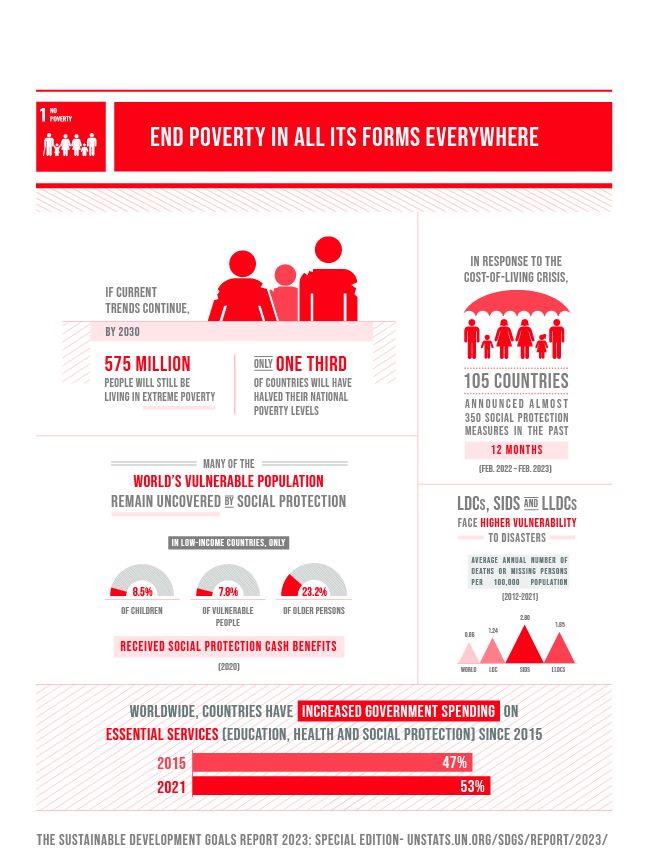
\includegraphics[width=0.4\linewidth]{reports/assignment-1/imgs/task2.jpg}
        \caption{Infographic on world poverty}
        \label{fig:viz}
    \end{figure}

    Figure \ref{fig:viz} shows the current trend for the development of the number of people living in poverty. It also shows how the poor are affected by poverty and how they are more vulnerable to disasters. On a lighter note, the infographic also shows that countries are taking concrete measures in order to reduce the number of people living in poverty.
    
    \item \begin{enumerate}
        \item Tufte's principles are:
        \begin{itemize}
            \item The five data-ink principles
            \begin{enumerate}
                \item Show the data
                \item Maximize the data-ink ratio, within reason
                \item Erase non-data ink, within reason
                \item Erase redundant data-ink
                \item Revise and edit
            \end{enumerate}
        \end{itemize}
        \item b
        \item c
        \item d
    \end{enumerate}
    
\end{enumerate}
\subsection{Dataset exploration}
\begin{enumerate}
    \item a
    \item b
\end{enumerate}

\bibliography{refs}

\end{document}
